\subsection{Cute Bunny}
    \subsubsection{Definición}
     \paragraph{El módulo \textbf{\emph{Cute Bunny}} es parte medular para la comunicación con otros sistemas. Cute Bunny es el encargado de proporcionar los respectivos servicios de tipo REST a otros sistemas o módulos que deseen consultar la información almacenada en las respectivas bases de tipo MX.}
  \paragraph{Cute Bunny interactúa con todos módulos de Ambienta2MX, Smart Owl, Hard Ant y Fast Eagle. La interacción con estos surge debido a que Hard Ant es el encargado de gestionar el acceso a las bases de datos de tipo MX y Smart Owl brindará y dará solución a las busquedas que no se encuentren en las bases de tipo MX, es decir, tratará de encontrar la información que Cute Bunny le solicitó para guardarla en algunas de las bases y posteriormente regresar el resultado al solicitante, en el caso de Fast Eagle, para la búsqueda de locaciones en la base de datos Places.}
      \begin{landscape}
        \subsubsection{Diagrama por bloques}
        \paragraph{A continuación se mostrará el diagrama por bloques que define la estructura de Cute Bunny.}
          \begin{figure}[b!]
          \centering
          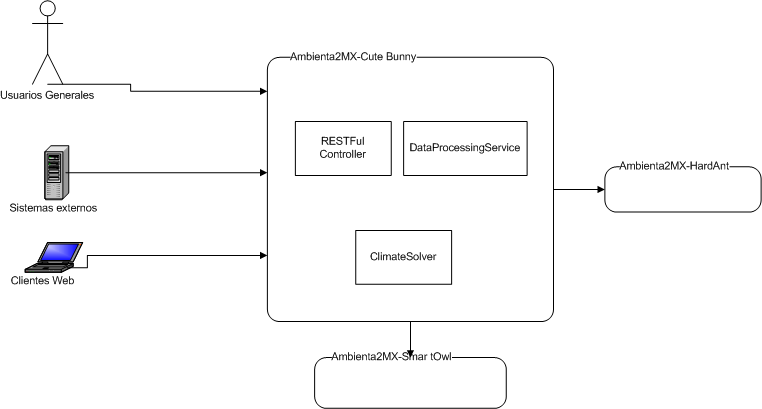
\includegraphics[width=22.5cm,height=12cm]{./images/DiagramaCuteBunny.png}
          \caption{Diagrama General de Cute Bunny}
        \end{figure}
      \end{landscape}
  \paragraph{La única función del módulo es comunicar y unificar los servicios generados, ya sea por SpringBoot(SmartOwl) o Vert.x (FastEagle y HardAnt). Esto con la finalidad de generar una API única que no requiera de que se acceda mediante distintas direcciones, con la finalidad de brindar una integración más rápida con las vistas generadas y gestionadas por el módulo Friendly Dolphin.}